\section{Operadores Diferenciais e Teoremas Integrais }

Vamos definir nesta se\c{c}\~ao os operadores diferenciais: gradiente,
divergente, rotacional e Laplace; e os teoremas integrais de Gauss e Stokes utilizando a
representa\c{c}\~ao tensorial apresentada nas se\c{c}\~oes anteriores.
\subsection {Coordenadas Cartesianas}

\begin{enumerate}

\item {\bf Operador Gradiente}\\
O operador gradiente pode ser escrito como
\begin{eqnarray}
\frac{\partial \Phi}{\partial x_{i}} = \Phi_{,i},
\end{eqnarray}
onde a v\ih rgula e o \ih ndice $i$ denotam a derivada com
rela\cao\ \`a coordenada espacial $x_{i}$. A nota\cao\ vetorial
deste operador pode ser $\nabla \Phi$ ou $\grad\Phi$.

\item {\bf Operador Divergente}\\
  Aplicado ao vetor $\vec{u}$, o operador divergente pode ser escrito
como
\begin{eqnarray}
\frac{\partial u_{i}}{\partial x_{i}} = u_{i,i} \, ,
\end{eqnarray}
e sua nota\cao\ vetorial \'e $\nabla\!\cdot\!\vec{u}$ ou $\divergent\vec{u}$.

\item {\bf Operador Rotacional}\\
Aplicado ao vetor $u$, o operador rotacional pode ser escrito
como
\begin{eqnarray}
\epsilon_{ijk}\frac{\partial }{\partial x_{j}}u_k =
\epsilon_{ijk}u_{k,\:j} \; ,
\end{eqnarray}
e sua nota\cao\ vetorial \'e $\nabla\!\times\!\vec{u}$, $\rot\vec{u}$ ou
    $\text{curl\thinspace}\vec{u}$.

\item {\bf Operador de Laplace (Laplaciano)}\\
\'E uma combina\cao\ do operador divergente com
o gradiente. Pode ser escrito como
\begin{eqnarray}
 \frac{\partial^{2}\Phi}{\partial x_{i}^2}= \frac{\partial^{2}\Phi}{\partial x_{i}\partial x_{i}} = \Phi_{,ii},
\end{eqnarray}
    tamb\'em existem outras nota\c{c}\~oes, dadas por $\Delta \Phi$ ou $\nabla^{2}\Phi$.
\\

\item{\bf Div rot e rot grad}\\
  Note que utilizando-se as representa\c{c}\~oes tensoriais e suas propriedades,
    podemos simplificar muito opera\c{c}\~oes do tipo $\nabla\cdot(\nabla\times\vec{u}) = 0$
    ou $\nabla\times(\nabla\Phi) = 0$, e.g.,
    \begin{align}
      \nabla\cdot(\nabla\times\vec{u}) &= (\epsilon_{ijk}u_{k,\thinspace j})_{,i}
      \, ,\\
      \nabla\cdot(\nabla\times\vec{u}) &= \epsilon_{ijk}u_{k,\thinspace ji} \, ,
      \\
      \nabla\cdot(\nabla\times\vec{u}) &= 0 \, ,
    \end{align}
    onde usamos a propriedade entre tensores sim\'etricos e o s\'imbolo de
    Levi-Civita, pois assumimos que $\frac{\partial}{\partial x_ix_j} =
    \frac{\partial}{\partial x_jx_i}$. Note que simplificamos muito a
    quantidade de opera\c{c}\~oes para chegar ao resultado final.
\\

\item {\bf Teorema de Gauss}\\
Mostra como transformar uma integral de volume numa integral de
superf\ih cie e vice versa,
\begin{eqnarray}
\int\!\!\!\int\!\!\!\int_{V_0} \mbox{div}\; \vec{u}\; dV = 
  \int\!\!\!\int_{\Sigma}\; \vec{u}\cdot\vec{n}\; dS \, ,
\end{eqnarray}
em sua forma tensorial
\begin{equation}
  \int\!\!\!\int\!\!\!\int_{V_0} u_{i,i}\; dV = 
  \int\!\!\!\int_{\Sigma}\; u_in_i \;dS \, ,
\end{equation}
onde $V_0$ \'e um volume envolvido pela superf\ih cie fechada
$\Sigma$ e $\vec{n}$ \'e um vetor normal externo unit\'ario de
$\Sigma$.

\item {\bf Teorema de Stokes}\\
Indica como transformar uma integral de superf\'icie em uma
integral de linha e vice versa,
\begin{eqnarray}
\int\!\!\!\int_{\Sigma}\vec{n}\cdot\mbox{rot}\; \vec{u}\; dS =
  \int_{L}\vec{u}\cdot\vec{t}\; dl\, ,
\end{eqnarray}
em sua forma tensorial
\begin{equation}
  \int\!\!\!\int_{\Sigma}n_i\,\epsilon_{ijk}u_{k,j}\; dS = \int_{L}u_it_i\; dl\,
  ,
\end{equation}
onde $\Sigma$ \'e uma superf\ih cie envolta por uma linha fechada
$L$ com um vetor tangente unit\'ario $\vec{t}$.

\end{enumerate}

\subsection {Coordenadas Ortogonais Curvil\'ineas}

A localiza\c{c}\~ao de um ponto no espa\c{c}o tridimensional
(com respeito a alguma origem) \'e normalmente especificada pelas
suas tr\^es coordenadas cartesianas ($x_1, x_2, x_3$) ou,
equivalentemente, ao especificar o vetor posi\c{c}ao do ponto.
Por\'em, existem situa\c{c}\~oes em que \'e mais conveniente
descrever a posi\c{c}\~ao do ponto por outro sistema
de coordenadas, mais apropriado para o problema em quest\~ao,
por exemplo, por coordenadas esf\'ericas ou cil\'indricas. Estes
exemplos, por sua vez, s\~ao casos espec\'ificos de sistemas
de coordenadas curvil\'ineas.

A rela\cao\ de transforma\cao\ entre coordenadas curvil\'ineas
$\gamma_{k}$ ($k = 1,2,3$) e coordenadas cartesianas pode ser
escrita como
\begin{eqnarray}
x_{i} = x_{i}(\gamma_{k})
\end{eqnarray}
ou
\begin{equation}
x_{i} = x_{i}(\gamma_{1}, \gamma_{2}, \gamma_{3}).
\end{equation}
Um elemento infinitesimal de comprimento ao longo do eixo $x_{i}$ \'e
\begin{eqnarray}
dx_{i} = \frac{\partial x_{i}}{\partial \gamma_{k}}d\gamma_{k}.
\end{eqnarray}
O comprimento de arco, $ds$, que \'e, basicamente, a dist\^ancia entre
dois pontos, \'e
\begin{eqnarray}
(ds)^{2} = dx_{i}dx_{i} = \frac{\partial x_{i}}{\partial
\gamma_{k}}\frac{\partial x_{i}}{\partial
\gamma_{l}}d\gamma_{k}d\gamma_{l} = g_{kl}d\gamma_{k}d\gamma_{l},
\label{eq:arclenght}
\end{eqnarray}
onde
\begin{eqnarray}
g_{kl} = \frac{\partial x_{i}}{\partial \gamma_{k}}\frac{\partial
x_{i}}{\partial \gamma_{l}}.
\end{eqnarray}
Temos coordenadas curvil\'ineas ortogonais quando $g_{kl} = 0$ para $k \neq l$,
ou seja, na situa\c{c}\~ao em que termos mistos n\~ao aparecem na express\~ao
do comprimento de arco (\ref{eq:arclenght}). Dizer que $g_{kl} = 0$ se $k \neq
l$, significa que
o vetor $\partial x_{i}$/$ \partial \gamma_{k}$ que \'e tangente a
$\gamma_{k}$, \'e ortogonal a $\partial x_{i}$/$\partial
\gamma_{l}$, tangente \`a coordenada $\gamma_{l}$. Ent\ao\
$\gamma_{k}$ e $\gamma_{l}$ s\ao\ ortogonais em qualquer ponto.
Nessa situa\c{c}\~ao temos
\begin{eqnarray}
(ds)^{2} = h_{1}^{2}(d\gamma_{1})^{2} + h_{2}^{2}(d\gamma_{2})^{2}
+ h_{3}^{2}(d\gamma_{3})^{2},
\end{eqnarray}
onde, por exemplo,
\begin{eqnarray}
h_{1}^{2} = \frac{\partial x_{1}}{\partial
\gamma_{1}}\frac{\partial x_{1}}{\partial \gamma_{1}} +
\frac{\partial x_{2}}{\partial \gamma_{1}}\frac{\partial
x_{2}}{\partial \gamma_{1}} + \frac{\partial x_{3}}{\partial
\gamma_{1}}\frac{\partial x_{3}}{\partial \gamma_{1}}.
\end{eqnarray}
\begin{figure}
\vspace{-2cm}
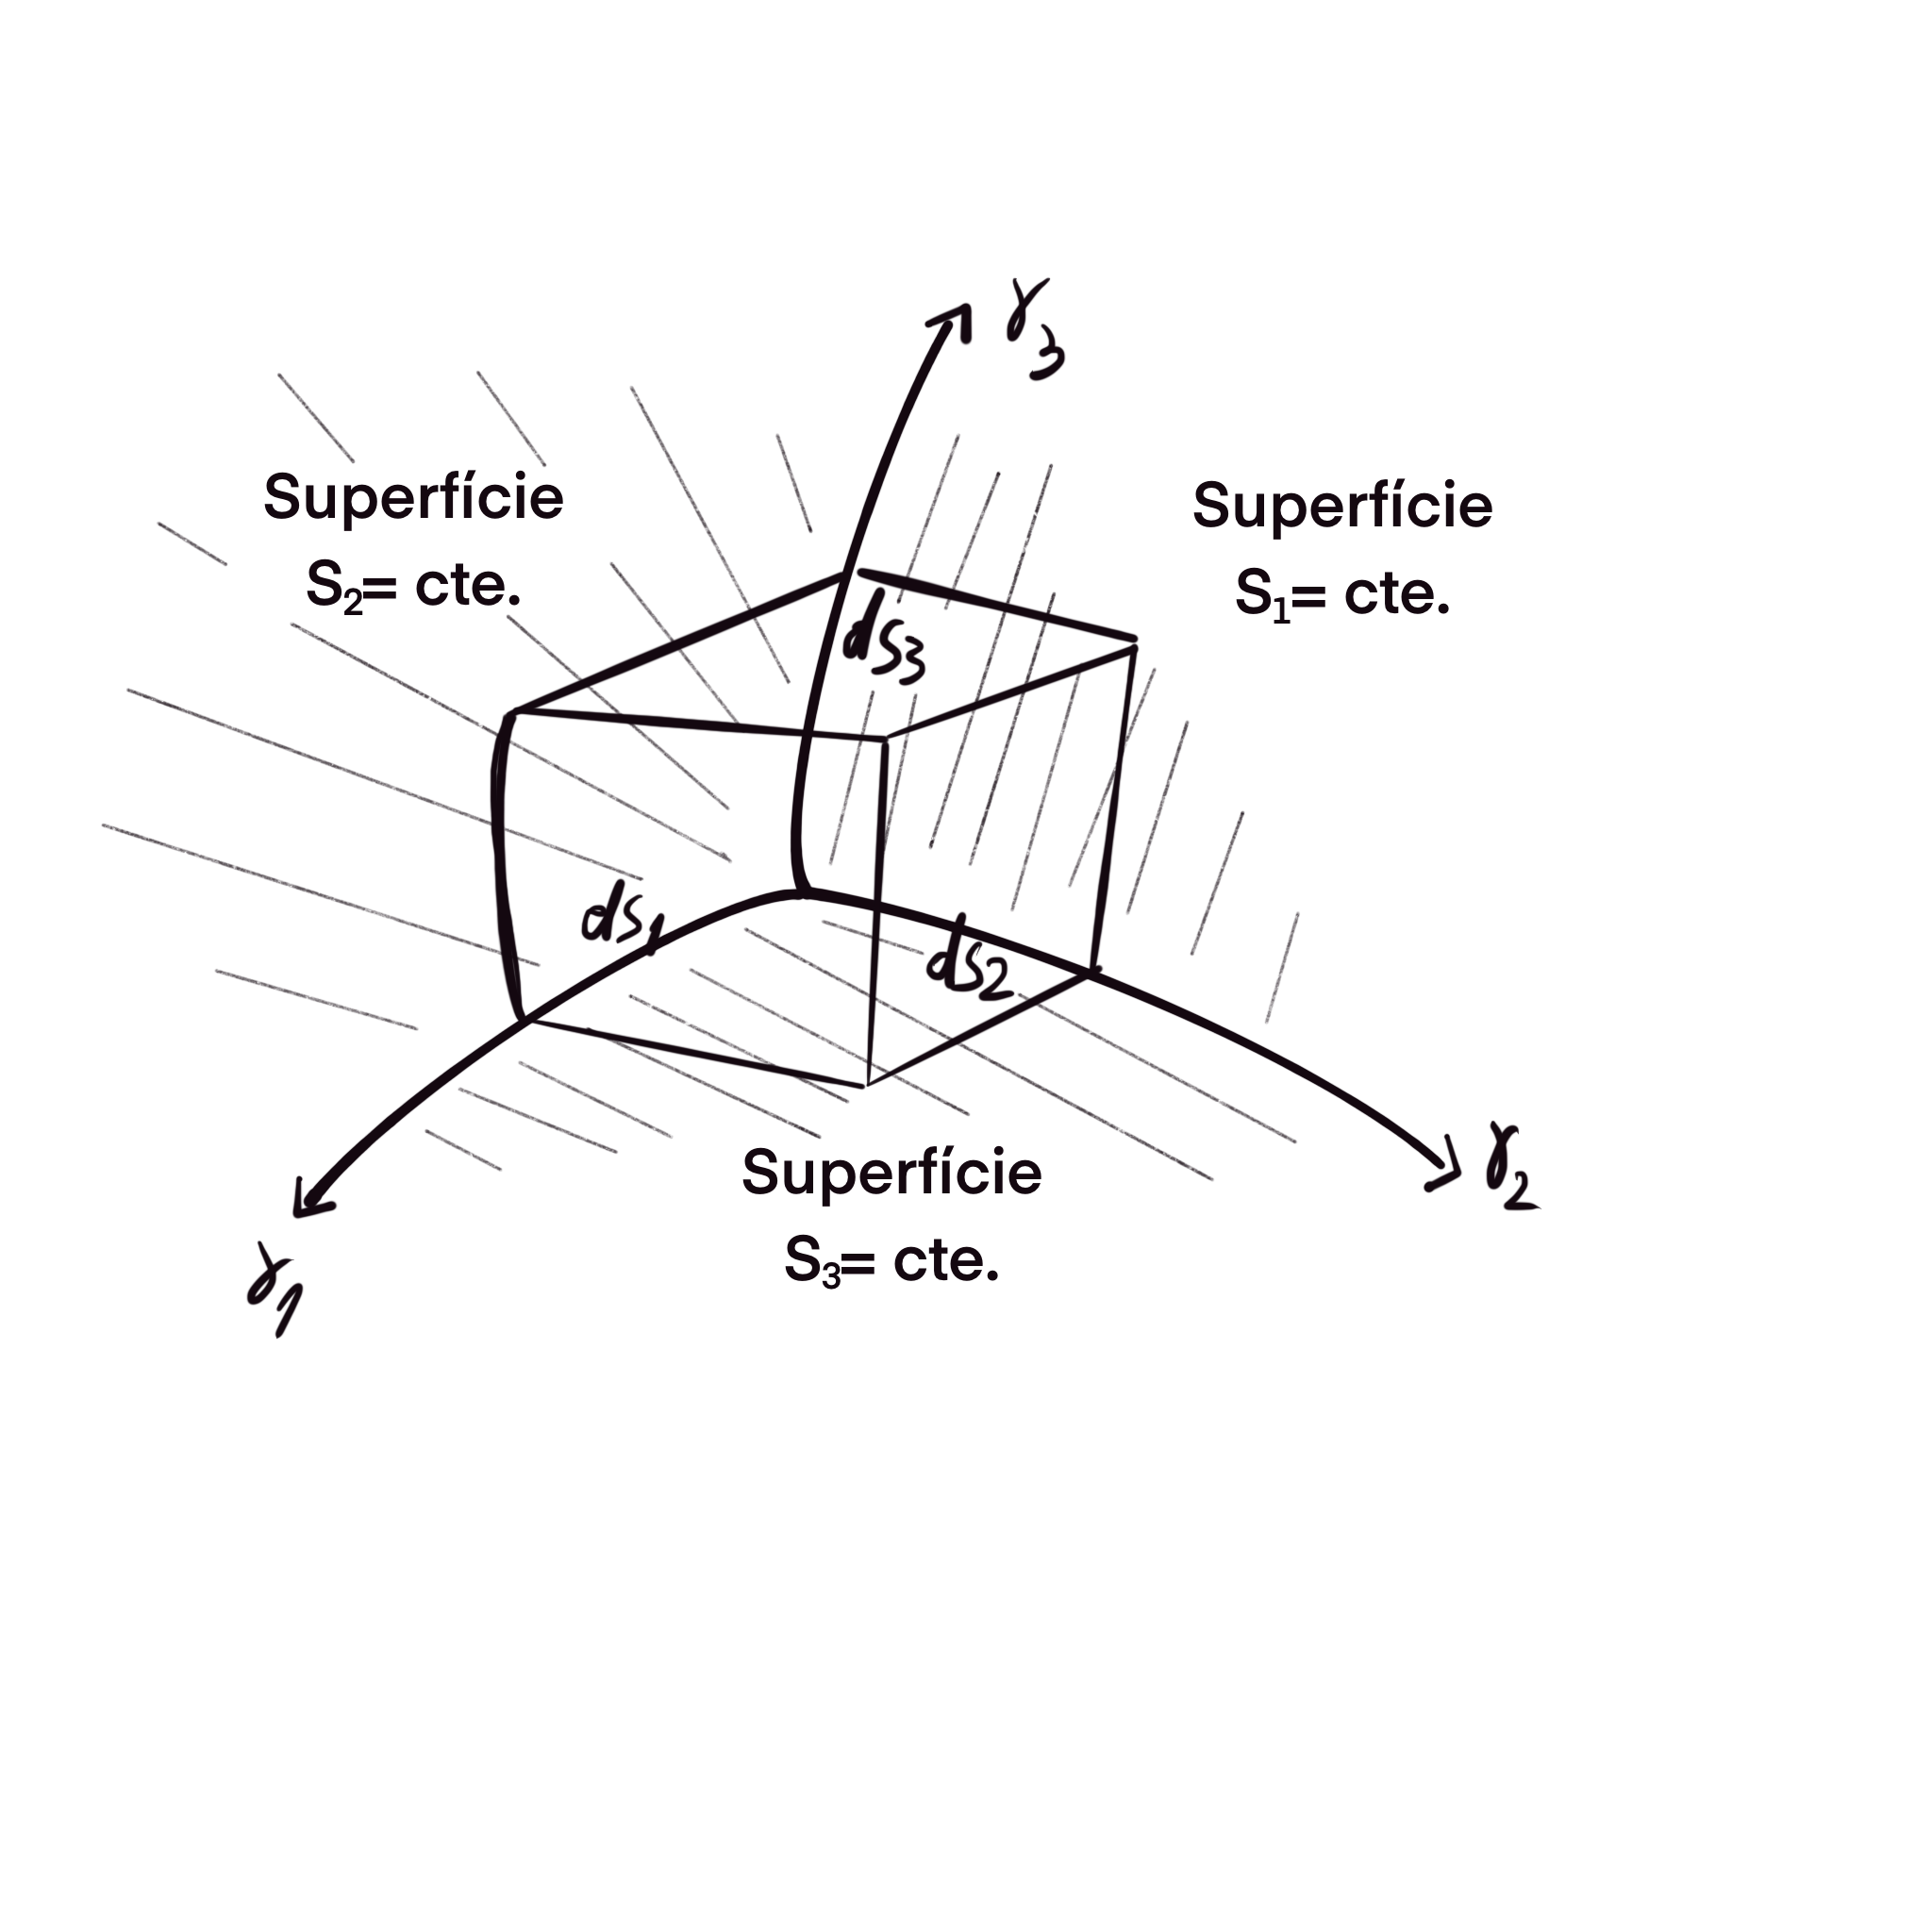
\includegraphics[width=1\columnwidth]{./figuras/sist-curv-ort1}
\vspace{-5.5cm}
\caption{Ilustra\c{c}\~ao de um sistema de coordenadas curvil\'ineas ortogonais.}
\label{fig:coord-curv-ort}
\end{figure}
Um elemento de comprimento ao longo de $\gamma_{1}$ (ver figura \ref{fig:coord-curv-ort}) \'e
\begin{eqnarray}
ds_{1} = h_{1}d\gamma_{1}
\end{eqnarray}
e similarmente, para comprimentos de onda ao longo dos outros eixos. Ent\~ao, podemos escrever
\begin{eqnarray}
\frac{\partial}{\partial s_{1}} \Leftrightarrow
\frac{1}{h_{1}}\frac{\partial}{\partial\gamma_{1}}.
\end{eqnarray}
Assim, o operador gradiente fica
\begin{eqnarray}
\nabla = \left(
\frac{1}{h_{1}}\frac{\partial}{\partial\gamma_{1}},
\frac{1}{h_{2}}\frac{\partial}{\partial\gamma_{2}},
\frac{1}{h_{3}}\frac{\partial}{\partial\gamma_{3}}\right).
\end{eqnarray}

%If for the moment we ascribe some constant value to qk> we have
Se assumirmos um valor constante para $\gamma_{k}$, temos
\begin{equation}
\gamma_{k}(x_1,x_2,x_3)=cte.,    %\hspace{2cm}   (k=1,2,3)
\end{equation}
%which describes a surface in space. By assigning a series of different values to qk, we generate a family of surfaces on which qk is constant.. If the func- tions have been properly chosen there is at least one surface belonging to each of the three families which passes through any arbitrary point P in space. Thus, a point in space is characterized by the intersection of the three surfaces, qj = constant, q2 = constant, q3 = constant (see Fig. A-I.I), termed coordinate surfaces. The coordinate surface is named for that co- ordinate which is constant, the other two coordinates being variable along
que descreve uma superf\'icie no espa\c{c}o (considerando que as outras coordenadas variam),
conhecida por superf\'icie coordenada.
A superf\'icie coordenada \'e nomeada pela coordenada com valor constante (ver figura \ref{fig:coord-curv-ort}).

Para encontrarmos o divergente e o laplaciano usamos o Teorema de Gauss
\begin{eqnarray}
\int\!\!\!\int\!\!\!\int_{V} u_{i,i}dV = \int\!\!\!\int_{S} u_{i}n_{i}dS
\end{eqnarray}
onde $n_{i}$ \'e vetor normal externo unit\'ario da superf\ih cie $S$ que envolve o volume $V$. 
Considere um sistema de coordenadas ortogonais curvil\ih neas $\gamma_{1}$,$\gamma_{2}$ e $\gamma_{3}$, 
e um volume elementar $dV = ds_{1}ds_{2}ds_{3}$ (figura \ref{fig:coord-curv-ort}).
As contribui\coes\ das superf\ih cies mais pr\'oximas aos eixos s\ao:
\begin{eqnarray}
-u_{1}ds_{2}ds_{3}, \; -u_{2}ds_{1}ds_{3}, \; -u_{3}ds_{1}ds_{2},
\end{eqnarray}
onde os sinais s\~ao negativos porque as orienta\coes\ dos vetores normais s\ao\ contr\'arias \`as dos eixos.
As contribui\coes\ das outras superf\ih cies s\ao:
\begin{eqnarray}
u_{1}ds_{2}ds_{3}+\frac{\partial}{\partial s_{1}}(u_{1}ds_{2}ds_{3})ds_{1},\\
u_{2}ds_{1}ds_{3}+\frac{\partial}{\partial s_{2}}(u_{2}ds_{1}ds_{3})ds_{2},\\
u_{3}ds_{1}ds_{2}+\frac{\partial}{\partial s_{3}}(u_{3}ds_{1}ds_{2})ds_{3}.
\end{eqnarray}
Somando as contribui\coes\ das seis faces e igualando \`a contribui\cao\ da integral de volume no Teorema de Gauss temos,
\begin{eqnarray}
u_{i,i} ds_1 ds_2 ds_3 &=& \frac{1}{h_1}\frac{\partial}{\partial \gamma_1} (h_2 h_3 u_1) d\gamma_2 d\gamma_3 ds_1 
 + \frac{1}{h_{2}}\frac{\partial}{\partial \gamma_{2}}(h_{1}h_{3}u_{2})d\gamma_{1}d\gamma_{3}ds_{2} \\ 
&+&\frac{1}{h_{3}}\frac{\partial}{\partial \gamma_{3}}(h_{1}h_{2}u_{3})d\gamma_{1}d\gamma_{2}ds_{3}
\end{eqnarray}
Usando $ds_{1} = h_{1}d\gamma_{1}$, etc., encontramos a express\~ao do divergente em coordenadas
ortogonais curvil\'ineas 
\begin{eqnarray}
u_{i,i}=\frac{1}{h_{1}h_{2}h_{3}}\left[\frac{\partial}{\partial\gamma_{1}}(h_{2}h_{3}u_{1}) 
       +\frac{\partial}{\partial \gamma_{2}}(h_{1}h_{3}u_{2})  
       +\frac{\partial}{\partial \gamma_{3}}(h_{1}h_{2}u_{3})\right].
\end{eqnarray}

Combinando as express\~oes para o gradiente e para o divergente em coordenadas curvil\ih neas ortogonais obtemos a express\ao\ para o 
Laplaciano $\Delta = \frac{\partial^{2}}{\partial x_{i}^{2}}$
\begin{eqnarray}
\Delta = \frac{1}{h_1 h_2 h_3}\left[\frac{\partial}{\partial\gamma_1}\left(\frac{h_2 h_3}{h_1}\frac{\partial}{\partial\gamma_1}\right)
+\frac{\partial}{\partial\gamma_{2}}\left(\frac{h_{1}h_{3}}{h_{2}}\frac{\partial}{\partial\gamma_{2}}\right)+
 \frac{\partial}{\partial\gamma_{3}}\left(\frac{h_{1}h_{2}}{h_{3}}\frac{\partial}{\partial\gamma_{3}}\right)\right].
\end{eqnarray}

\section{Sinal Anal\ih tico}

A fun\cao\ sinal anal\ih tico $F(\xi)$ \'e definida como
\begin{eqnarray}
F(\xi) = g(\xi) + ih(\xi)
\end{eqnarray}
e ser\'a usada no estudo de ondas transientes. Aqui $g(\xi)$ \'e o
sinal transiente real para o qual o sinal anal\ih tico \'e
constru\ih do e $h(\xi)$ \'e a transformada de Hilbert de
$g(\xi)$,
\begin{eqnarray}
h(\xi) =
\frac{1}{\pi}\int_{-\infty}^{\infty}\frac{g(\sigma)}{\sigma-\xi}d\sigma,
\end{eqnarray}
onde $g(\xi)$ e $h(\xi)$ formam um par da transformada de Hilbert.
Antes de entrar na discuss\ao\ do sinal anal\ih tico na teoria de
propaga\cao\ de ondas planas transientes, vejamos alguns fatos
importantes da an\'alise de Fourier. Considerando o grupo de
fun\coes\ de Fourier do tipo padr\ao, que s\ao\ as absolutamente
integr\'aveis em $(-\infty,\infty)$ e satisfazem as condi\coes\ de
Dirichlet num intervalo finito. Uma fun\cao\ \'e dita
absolutamente integr\'avel se
\begin{eqnarray}
\int_{-\infty}^{\infty}\mid g(t)\mid dt \leq A,
\end{eqnarray}
onde $A$ \'e uma constante real positiva. A condi\cao\ de
Dirichlet requer a continuidade de $g(\xi)$ em um intervalo finito
com a possibilidade de finitas descontinuidades do primeiro tipo
(onde existem limites finitos \`a esquerda e \`a direita), e
n\'umero finito de m\'aximos e m\ih nimos. Sob essas codi\coes\ a
transformada de Fourier \'e definida como
\begin{eqnarray}
\hat{g}(\omega) = \int_{-\infty}^{\infty}g(t)e^{i 2 \pi \omega t}dt,\; g(t) =
\int_{-\infty}^{\infty}\hat{g}(\omega)e^{-i 2 \pi \omega t}d\omega
\end{eqnarray}
Para explica\c{c}\~oes futuras, precisaremos saber o teorema da
convolu\c{c}\~ao e a inversa da transformada de Fourier da fun\c{c}\~ao
sinal - $sgn(\omega)$. 

A convolu\c{c}\~ao $c(t)$ de duas fun\c{c}\~oes, $a(t)$ e $b(t)$ \'e dada por
\begin{eqnarray}
c(t) = \int_{-\infty}^{\infty} a(\tau)b(t-\tau)d\tau,
\end{eqnarray}
simbolicamente escrita como $c(t) = a(t)*b(t)$. O teorema da
convolu\cao\ diz que a transformada de Fourier da convolu\cao\
\'e igual ao produto das transformadas das fun\coes\ $a(t)$ e
$b(t)$,
\begin{eqnarray}
c(\omega) = a(\omega)b(\omega).
\end{eqnarray}

A fun\cao\ sinal \'e definida como
\begin{eqnarray}
\sgn(\omega) = \left\{
\begin{array}{ll}
1 , \omega > 0 \\
0 , \omega = 0 \\
-1 , \omega < 0
\end{array}
\right.
\end{eqnarray}
Como esta fun\cao\ n\ao\ \'e absolutamente integr\'avel, \'e
preciso achar a inversa da transformada de Fourier como um caso
limite de uma fun\cao\ auxiliar que no limite se aproxima da
fun\cao\ $\sgn(\omega)$. Esta fun\cao\ pode ser
\begin{eqnarray}
\hat{g}_{\alpha}(\omega) = e^{-\alpha \mid \omega\mid}i \sgn(\omega)
\end{eqnarray}
com $\alpha > 0$. Esta \'e uma fun\cao\ integr\'avel e quando
$\alpha\rightarrow 0$ a fun\cao\ se aproxima de $i$ $\sgn(\omega)$.
Ent\ao\ basta tomar a transformada de Fourier inversa e fazer
$\alpha\rightarrow 0$ para obter a transformada inversa de $i\sgn(\omega)$.
%\begin{equation}
\begin{multline}
g_{\alpha}(t) = \int_{-\infty}^{\infty}e^{-\alpha \mid
\omega \mid}i\sgn(\omega)e^{-i2\pi \omega t}d\omega \\
= -\int_{-\infty}^{0}e^{\alpha \omega}e^{-i2\pi \omega t}i d\omega +
\int_{0}^{\infty}e^{-\alpha \omega}e^{-i2\pi \omega t}i d\omega \\
= -\int_{0}^{\infty}e^{-\alpha \omega^{'}}e^{i2\pi \omega^{'}t}i d\omega^{'} +
\int_{0}^{\infty}e^{-(\alpha+i2\pi t)\omega}i d\omega \\
= -\int_{0}^{\infty}e^{(-\alpha+2i\pi t)\omega}i d\omega +
\int_{0}^{\infty}e^{-(\alpha + 2i\pi t)\omega}i d\omega \\
= \frac{i}{i2\pi t - \alpha} + \frac{i}{i2\pi t + \alpha}.
\end{multline}
%\end{equation}
Para $\alpha\rightarrow 0$ temos
\begin{eqnarray}
g_{\alpha}(t)\rightarrow g_{0}(t) = \int_{-\infty}^{\infty}i\sgn(\omega)e^{-i2\pi \omega t}dt =
\frac{1}{\pi t}.
\end{eqnarray}
Temos ent\ao\ um par de Fourier
\begin{eqnarray}
g_{0}(t) = (\pi t)^{-1},\; \hat{g}_{0}(\omega) = i\sgn(\omega).
\end{eqnarray}

Sabemos que, para uma fun\cao\ real $g(t)$
\begin{eqnarray}
\hat{g}^{*}(\omega) = \int_{-\infty}^{\infty}g(t)e^{-i2\pi \omega t}dt = \hat{g}(-\omega).
\end{eqnarray}
Usando esta propriedade e sabendo que, sendo o n\'umero complexo
$z=x+yi$ e $2Re(z)=z+\bar{z}$,
reescrevemos a express\~ao para o sinal real da seguinte maneira
\begin{multline}
g(t) = \int_{-\infty}^{\infty}\hat{g}(\omega)e^{-i2\pi \omega t}d\omega \\
= \int_{-\infty}^{0}\hat{g}(\omega)e^{-i2\pi \omega t}d\omega +
\int_{0}^{\infty}\hat{g}(\omega)e^{-i2\pi \omega t}d\omega \\
= \int_{0}^{\infty}\hat{g}(-\omega)e^{i2\pi \omega t}d\omega +
\int_{0}^{\infty}
\hat{g}(\omega)e^{-i2\pi \omega t}d\omega \\
= \int_{0}^{\infty}\hat{g}^{*}(\omega)e^{i2\pi \omega t}d\omega +
\int_{0}^{\infty}\hat{g}(\omega)e^{-i2\pi \omega t}d\omega \\
= 2Re\{ \int_{0}^{\infty}\hat{g}(\omega)e^{-i2\pi \omega t}d\omega \} .
\end{multline}
Ent\ao,
\begin{equation}
\begin{split}
g(t) = 2Re\{ \int_{0}^{\infty}\hat{g}(\omega)e^{-i2\pi \omega t}d\omega \} \\
= Re\{2 \int_{0}^{\infty}\hat{g}(\omega)e^{-i2\pi \omega t}d\omega \}
\end{split}
\end{equation}
Assim, como vemos, $g(t)$ \'e a parte real do sinal complexo
\begin{eqnarray}
F(t) = 2\int_{0}^{\infty}\hat{g}(\omega)e^{-i2\pi \omega t}d\omega,
\end{eqnarray}
que tamb\'em pode ser escrito como
\begin{eqnarray}
F(t) = g(t) + ih(t),
\label{sinan}
\end{eqnarray}
Mas quem \'e a parte imagin\'aria $h(t)$ deste sinal complexo?
Sabendo que, sendo $z$ um n\'umero complexo, $Im(z)=(z+\bar{z})/2i$, ent\~ao %onde
%\begin{eqnarray}
%h(t) = 2Im\{ \int_{0}^{\infty}\hat{g}(\omega)e^{-i2\pi \omega t}d\omega \}.
%\end{eqnarray}
\begin{equation}
h(t)=Im\{F(t)\} = \frac{F(t) - F^*(t)}{2i}
\end{equation}
Encontrando $h(t)$:
\begin{eqnarray}
h(t) &=& \frac{1}{i}\left[\int_{0}^{\infty}\hat{g}(\omega)e^{-i2\pi \omega t}d\omega -
\int_{0}^{\infty}\hat{g}(-\omega)e^{i2\pi \omega t}d\omega  \right]\nonumber \\
&=& \frac{1}{i}\left[\int_{0}^{\infty}\hat{g}(\omega)e^{-i2\pi \omega t}d\omega -
\int_{-\infty}^{0}\hat{g}(\omega)e^{-i2\pi \omega t}d\omega  \right]\nonumber \\
&=& \int_{-\infty}^{\infty}\hat{g}(\omega) [-i\sgn(\omega)]e^{-i2\pi \omega t}d\omega
\nonumber \\
&=& g(t) * \frac{1}{\pi t}\nonumber \\
&=&
\frac{1}{\pi}\int_{-\infty}^{\infty}\frac{g(\tau)}{t-\tau}d\tau
\nonumber \\
&=& \frac{1}{\pi}\int_{-\infty}^{\infty}\frac{g(\tau)}{t -
\tau}d\tau.
\label{thil}
\end{eqnarray}

Ent\ao\ $g(t)$ e $h(t)$ formam um par de Hilbert, isto \'e, $h(t)$ \'e
a transformada de Hilbert de $g(t)$. O sinal complexo (\ref{sinan})
\'e o sinal anal\ih tico.


Devemos observar que a Transformada de Hilbert da Transformada de
Hilbert de um sinal $g(t)$ fornece $-g(t)$, ou seja,
\begin{equation}
g(t) = - \frac{1}{\pi} \int_{-\infty}^{\infty} \frac{h(\xi)}{\xi-t}d\xi
= \frac{1}{\pi} \int_{-\infty}^{\infty} \frac{h(\xi)}{t-\xi}d\xi \; .
\label{thth}
\end{equation}
Isso pode ser provado usando o sinal anal\itico\ $Y(t) = -iF(t) = -i
(g(t) + ih(t)) = h(t) - i g(t)$. Usando o mesmo racioc\inio\ das equa\coes\
(\ref{thil}), mostra-se que $-g(t)=Im \{Y(t)\}$ \'e a transformada de
Hilbert de $h(t)=Re\{Y(t)\}$.

Um importante par de Hilbert e seu correspondente sinal anal\ih
tico est\'a relacionado ao sinal real na forma da fun\cao\
$\delta$ de Dirac. Para $g(t) = \delta(t)$, a equa\cao\ para
$h(t)$ fica
\begin{eqnarray}
h(t) = \int_{-\infty}^{\infty}\frac{\delta(\sigma)}{\sigma - t}d\delta
= -\frac{1}{\pi t}.
\end{eqnarray}
O correspondente sinal anal\ih tico tem a forma
\begin{eqnarray}
F(t) = \delta(t) - \frac{i}{\pi t}.
\end{eqnarray}

Uma propriedade importante da transformada de Hilbert \'e que a
transformada de Hilbert da derivada $dg(t)/dt$ \'e a derivada
$dh(t)/dt$ da transformada de Hilbert do sinal $g(t)$.
\begin{eqnarray}
\frac{dh(t)}{dt} &=& 2Im\int_{0}^{\infty}g(f)(-i2\pi f)e^{-i2\pi
ft}df, \\
\frac{dg(t)}{dt} &=& 2Re\int_{0}^{\infty}g(f)(-i2\pi f)e^{-i2\pi
ft}df.
\end{eqnarray}
Da primeira equa\cao\ vemos que a derivada da transformada de
Hilbert $h(t)$ corresponde a um "novo" sinal cuja transformada de
Fourier \'e $g(f)(-i2\pi f)$. Da segunda equa\cao\ vemos que o
"novo" sinal \'e $dg(t)/dt$.


%\begin{thebibliography}{99}
%\bibitem{Psencik} P\v{s}en\v{c}ik, I., 1994, {\em Introduction to seismic
%methods - Lecture Notes}, PPPG / UFBa.
%\end{thebibliography}

